\documentclass{beamer}
\usepackage[utf8]{inputenc}
\usepackage{amsmath,amssymb}
\usepackage{graphicx}
\usepackage{epstopdf}
\usepackage[listings,theorems]{tcolorbox}
\usepackage{tikz}
\usepackage{pgf}
\usepackage[customcolors,shade]{hf-tikz}
\usefonttheme{serif} % default family is serif
\setbeamersize{text margin left=5mm,text margin right=5mm} 

\usetikzlibrary{positioning,shapes}
\usetikzlibrary{shapes.geometric,arrows,automata,tikzmark}
\usetikzlibrary{arrows,decorations.pathmorphing}
\tikzstyle{io} = [trapezium, trapezium left angle=70, trapezium right angle=110, minimum width=3cm, minimum height=1cm, text centered, draw=black, fill=blue!30]
\tikzstyle{process} = [rectangle, minimum width=3cm, minimum height=1cm, text centered, draw=black, fill=orange!30]
\tikzstyle{decision} = [diamond, minimum width=3cm, minimum height=1cm, text centered, draw=black, fill=green!30]
\tikzstyle{arrow} = [thick,->,>=stealth]

%Information to be included in the title page:
\title{Optimización de la estructura electrónica del átomo de Be}
\author{A. Mendez}
%\institute{Overleaf}
\date{\today} % It's always today!

\begin{document}
\frame{\titlepage}
%%%%%%%%%%%%%%%%%%%%%%%%%%%%%%%%%%%%%%%%%%%%%%%%%%%%%%%%%%%%%%%%%%%%%%%%
\begin{frame}[t]
\frametitle{Algunas variables importantes en la optimización de Be}
\begin{itemize}
\item Configuraciones en CI 
  \begin{itemize}
    \item[ ] $\rightarrow$ $N$ parámetros
  \end{itemize}
\item Potencial modelo $V_{nl}^{\textrm{eff}}(r)$ 
  \begin{itemize}
    \item[ ] $\rightarrow$ Tipo de potencial: TFDA o STO
    \item[ ] $\rightarrow$ $nl$ parámetros: $\boldsymbol{\lambda}_{nl}$ 
  \end{itemize}
\item Potencial de polarización $V_l^{\textrm{pol}}(r)$ 
  \begin{itemize}
    \item[ ] $\rightarrow$ Tipo de potencial: Norcross o Bayliss
    \item[ ] $\rightarrow$ $2(l+1)$ parámetros: $\boldsymbol{\xi}_l=\{\alpha_l,\rho_l$\} 
  \end{itemize}
\end{itemize}
\end{frame}
%%%%%%%%%%%%%%%%%%%%%%%%%%%%%%%%%%%%%%%%%%%%%%%%%%%%%%%%%%%%%%%%%%%%%%%%
\begin{frame}[t]
\frametitle{Parámetros de la optimización}

\begin{itemize}
\item Espacio de hiper-parámetros
\item Diseño inicial
  \begin{itemize}
    \item Tipo de mapeo (random, latin hypercube, etc.)
    \item Número de datos iniciales
  \end{itemize}
\item Kernel (squared exponential, periodic, etc.)
\item Función de adquisión (EI, MPI, etc.)
\item Presupuesto (máximo número de evaluaciones)
\item Función costo: 
  \begin{itemize}
    \item Suma de errores relativos de energías absolutas de $n$ niveles
    \item Suma de errores relativos de coeficientes de Einstein de $t$ transiciones
  \end{itemize}
\end{itemize}

\begin{center}
¿Cómo saber si el mínimo hallado en una optimización \\ es el mínimo global?

\medskip
\color{red}{
$\rightarrow$ Evaluación del modelo usando 100 semillas diferentes $\leftarrow$}
\end{center}

\end{frame}
%%%%%%%%%%%%%%%%%%%%%%%%%%%%%%%%%%%%%%%%%%%%%%%%%%%%%%%%%%%%%%%%%%%%%%%%
\begin{frame}[t]
\frametitle{Potencial de polarización}

\begin{itemize}
\item Número de configuraciones en CI: \texttt{mxconf=6}
\item Potencial de Norcross (1976)
\vspace{-0.25cm}
\begin{equation*}
  V_{\textrm{pol}}(r) = -\frac{\alpha_l}{r^4}\left[1-e^{-\left(\tfrac{r}{\rho_l}\right)^6}\right]
\end{equation*}
\vspace{-0.6cm}
\item Espacio de hiper--parámetros: \texttt{npolvar=6}
  \vspace{-0.25cm}
  \begin{align*} 
    \alpha_l &=[0.0010,0.2000] \\
    \rho_l   &=[0.2000,1.5000] \quad:\quad l=0,1,2
  \end{align*}
\vspace{-0.8cm}
\item Diseño inicial:
  \begin{itemize}
    \item Tipo de mapeo (random, latin hypercube, etc.)
    \item Número de datos iniciales: \texttt{initer}
  \end{itemize}
\item Kernel: RBF (squared exponential)
\item Función de adquisión: EI
\item Presupuesto: \texttt{maxeval}
\item Función costo: $\sum_i (E_i^{\textrm{obs.}}-E_i^{\textrm{comp.}})/E_i^{\textrm{obs.}})$
\end{itemize}

%\begin{tikzpicture}[remember picture, overlay]
% \tikzset{shift={(current page.center)},xshift=0cm,yshift=0cm}
%\end{tikzpicture}

\end{frame}
%%%%%%%%%%%%%%%%%%%%%%%%%%%%%%%%%%%%%%%%%%%%%%%%%%%%%%%%%%%%%%%%%%%%%%%%
\begin{frame}
\frametitle{Estudio de mapeo inicial:}

\begin{tikzpicture}[remember picture, overlay]
 \tikzset{shift={(current page.center)},xshift=0cm,yshift=0cm}
%%%%%%%%%%%%%%%%%%%%
 \node<1> at (0,3.5) {\texttt{initer=12}};
 \node<1> at (-3.8,2.6) {Random};
 \node<1> at (-4,1.4) {\includegraphics[trim={0 0 0 0.5cm},clip,width=0.33\textwidth]{figures/pol_conv/initer12/maxevals0/Jmin_random.eps}};
 \node<1> at (0,1.4) {\includegraphics[trim={0 0 0 0.5cm},clip,width=0.33\textwidth]{figures/pol_conv/initer12/maxevals0/imin_random.eps}};
 \node<1> at (4,1.4) {\includegraphics[trim={0 0 0 0},clip,width=0.33\textwidth]{figures/pol_conv/initer12/maxevals0/minspace_random.eps}};
 \node<1> at (-3.9,-1.3) {Latin};
 \node<1> at (-4,-2.5) {\includegraphics[trim={0 0 0 0.5cm},clip,width=0.33\textwidth]{figures/pol_conv/initer12/maxevals0/Jmin_latin.eps}};
 \node<1> at (0,-2.5) {\includegraphics[trim={0 0 0 0.5cm},clip,width=0.33\textwidth]{figures/pol_conv/initer12/maxevals0/imin_latin.eps}};
 \node<1> at (4,-2.5) {\includegraphics[trim={0 0 0 0},clip,width=0.33\textwidth]{figures/pol_conv/initer12/maxevals0/minspace_latin.eps}};
%%%%%%%%%%%%%%%%%%%%
 \node<2> at (0,3.5) {\texttt{initer=24}};
 \node<2> at (-3.8,2.6) {Random};
 \node<2> at (-4,1.4) {\includegraphics[trim={0 0 0 0.5cm},clip,width=0.33\textwidth]{figures/pol_conv/initer24/maxevals0/Jmin_random.eps}};
 \node<2> at (0,1.4) {\includegraphics[trim={0 0 0 0.5cm},clip,width=0.33\textwidth]{figures/pol_conv/initer24/maxevals0/imin_random.eps}};
 \node<2> at (4,1.4) {\includegraphics[trim={0 0 0 0},clip,width=0.33\textwidth]{figures/pol_conv/initer24/maxevals0/minspace_random.eps}};
 \node<2> at (-3.9,-1.3) {Latin};
 \node<2> at (-4,-2.5) {\includegraphics[trim={0 0 0 0.5cm},clip,width=0.33\textwidth]{figures/pol_conv/initer24/maxevals0/Jmin_latin.eps}};
 \node<2> at (0,-2.5) {\includegraphics[trim={0 0 0 0.5cm},clip,width=0.33\textwidth]{figures/pol_conv/initer24/maxevals0/imin_latin.eps}};
 \node<2> at (4,-2.5) {\includegraphics[trim={0 0 0 0},clip,width=0.33\textwidth]{figures/pol_conv/initer24/maxevals0/minspace_latin.eps}};
%%%%%%%%%%%%%%%%%%%%
 \node<3> at (0,3.5) {\texttt{initer=36}};
 \node<3> at (-3.8,2.6) {Random};
 \node<3> at (-4,1.4) {\includegraphics[trim={0 0 0 0.5cm},clip,width=0.33\textwidth]{figures/pol_conv/initer36/maxevals0/Jmin_random.eps}};
 \node<3> at (0,1.4) {\includegraphics[trim={0 0 0 0.5cm},clip,width=0.33\textwidth]{figures/pol_conv/initer36/maxevals0/imin_random.eps}};
 \node<3> at (4,1.4) {\includegraphics[trim={0 0 0 0},clip,width=0.33\textwidth]{figures/pol_conv/initer36/maxevals0/minspace_random.eps}};
 \node<3> at (-3.9,-1.3) {Latin};
 \node<3> at (-4,-2.5) {\includegraphics[trim={0 0 0 0.5cm},clip,width=0.33\textwidth]{figures/pol_conv/initer36/maxevals0/Jmin_latin.eps}};
 \node<3> at (0,-2.5) {\includegraphics[trim={0 0 0 0.5cm},clip,width=0.33\textwidth]{figures/pol_conv/initer36/maxevals0/imin_latin.eps}};
 \node<3> at (4,-2.5) {\includegraphics[trim={0 0 0 0},clip,width=0.33\textwidth]{figures/pol_conv/initer36/maxevals0/minspace_latin.eps}};
%%%%%%%%%%%%%%%%%%%%
 \node<4> at (0,3.5) {\texttt{initer=48}};
 \node<4> at (-3.8,2.6) {Random};
 \node<4> at (-4,1.4) {\includegraphics[trim={0 0 0 0.5cm},clip,width=0.33\textwidth]{figures/pol_conv/initer48/maxevals0/Jmin_random.eps}};
 \node<4> at (0,1.4) {\includegraphics[trim={0 0 0 0.5cm},clip,width=0.33\textwidth]{figures/pol_conv/initer48/maxevals0/imin_random.eps}};
 \node<4> at (4,1.4) {\includegraphics[trim={0 0 0 0},clip,width=0.33\textwidth]{figures/pol_conv/initer48/maxevals0/minspace_random.eps}};
 \node<4> at (-3.9,-1.3) {Latin};
 \node<4> at (-4,-2.5) {\includegraphics[trim={0 0 0 0.5cm},clip,width=0.33\textwidth]{figures/pol_conv/initer48/maxevals0/Jmin_latin.eps}};
 \node<4> at (0,-2.5) {\includegraphics[trim={0 0 0 0.5cm},clip,width=0.33\textwidth]{figures/pol_conv/initer48/maxevals0/imin_latin.eps}};
 \node<4> at (4,-2.5) {\includegraphics[trim={0 0 0 0},clip,width=0.33\textwidth]{figures/pol_conv/initer48/maxevals0/minspace_latin.eps}};
%%%%%%%%%%%%%%%%%%%%
 \node<5> at (0,3.5) {\texttt{initer=60}};
 \node<5> at (-3.8,2.6) {Random};
 \node<5> at (-4,1.4) {\includegraphics[trim={0 0 0 0.5cm},clip,width=0.33\textwidth]{figures/pol_conv/initer60/maxevals0/Jmin_random.eps}};
 \node<5> at (0,1.4) {\includegraphics[trim={0 0 0 0.5cm},clip,width=0.33\textwidth]{figures/pol_conv/initer60/maxevals0/imin_random.eps}};
 \node<5> at (4,1.4) {\includegraphics[trim={0 0 0 0},clip,width=0.33\textwidth]{figures/pol_conv/initer60/maxevals0/minspace_random.eps}};
 \node<5> at (-3.9,-1.3) {Latin};
 \node<5> at (-4,-2.5) {\includegraphics[trim={0 0 0 0.5cm},clip,width=0.33\textwidth]{figures/pol_conv/initer60/maxevals0/Jmin_latin.eps}};
 \node<5> at (0,-2.5) {\includegraphics[trim={0 0 0 0.5cm},clip,width=0.33\textwidth]{figures/pol_conv/initer60/maxevals0/imin_latin.eps}};
 \node<5> at (4,-2.5) {\includegraphics[trim={0 0 0 0},clip,width=0.33\textwidth]{figures/pol_conv/initer60/maxevals0/minspace_latin.eps}};
\end{tikzpicture}

\end{frame}
%%%%%%%%%%%%%%%%%%%%%%%%%%%%%%%%%%%%%%%%%%%%%%%%%%%%%%%%%%%%%%%%%%%%%%%%
\begin{frame}[t]
\frametitle{Conclusión:}

\begin{itemize}
 \item Latin hypercube es la mejor herramienta para hacer el muestreo inicial.
 \item El número de elementos en el muestreo inicial \texttt{initer} es crucial para reducir 
el valor máximo que puede tomar la función de costo.
\end{itemize}

\end{frame}
%%%%%%%%%%%%%%%%%%%%%%%%%%%%%%%%%%%%%%%%%%%%%%%%%%%%%%%%%%%%%%%%%%%%%%%%
\begin{frame}
\frametitle{Estudio de presupuesto vs mapeo inicial:}

\begin{tikzpicture}[remember picture, overlay]
 \tikzset{shift={(current page.center)},xshift=0cm,yshift=0cm}
 \node<1-> at (-3.8,2.6) {\texttt{maxeval=12}};
 \node<1-> at (-3.8,-1.3) {\texttt{maxeval=0}};
%%%%%%%%%%%%%%%%%%%%
 \node<1> at (0,3.5) {\texttt{initer=12}};
 \node<1> at (-4,1.4) {\includegraphics[trim={0 0 0 0.5cm},clip,width=0.33\textwidth]{figures/pol_conv/initer12/maxevals12/Jmin_latin.eps}};
 \node<1> at (0,1.4) {\includegraphics[trim={0 0 0 0.5cm},clip,width=0.33\textwidth]{figures/pol_conv/initer12/maxevals12/imin_latin.eps}};
 \node<1> at (4,1.4) {\includegraphics[trim={0 0 0 0},clip,width=0.33\textwidth]{figures/pol_conv/initer12/maxevals12/minspace_latin.eps}};
 \node<1> at (-4,-2.5) {\includegraphics[trim={0 0 0 0.5cm},clip,width=0.33\textwidth]{figures/pol_conv/initer12/maxevals0/Jmin_latin.eps}};
 \node<1> at (0,-2.5) {\includegraphics[trim={0 0 0 0.5cm},clip,width=0.33\textwidth]{figures/pol_conv/initer12/maxevals0/imin_latin.eps}};
 \node<1> at (4,-2.5) {\includegraphics[trim={0 0 0 0},clip,width=0.33\textwidth]{figures/pol_conv/initer12/maxevals0/minspace_latin.eps}};
%%%%%%%%%%%%%%%%%%%%
 \node<2> at (0,3.5) {\texttt{initer=24}};
 \node<2> at (-4,1.4) {\includegraphics[trim={0 0 0 0.5cm},clip,width=0.33\textwidth]{figures/pol_conv/initer24/maxevals12/Jmin_latin.eps}};
 \node<2> at (0,1.4) {\includegraphics[trim={0 0 0 0.5cm},clip,width=0.33\textwidth]{figures/pol_conv/initer24/maxevals12/imin_latin.eps}};
 \node<2> at (4,1.4) {\includegraphics[trim={0 0 0 0},clip,width=0.33\textwidth]{figures/pol_conv/initer24/maxevals12/minspace_latin.eps}};
 \node<2> at (-4,-2.5) {\includegraphics[trim={0 0 0 0.5cm},clip,width=0.33\textwidth]{figures/pol_conv/initer24/maxevals0/Jmin_latin.eps}};
 \node<2> at (0,-2.5) {\includegraphics[trim={0 0 0 0.5cm},clip,width=0.33\textwidth]{figures/pol_conv/initer24/maxevals0/imin_latin.eps}};
 \node<2> at (4,-2.5) {\includegraphics[trim={0 0 0 0},clip,width=0.33\textwidth]{figures/pol_conv/initer24/maxevals0/minspace_latin.eps}};
%%%%%%%%%%%%%%%%%%%
 \node<3> at (0,3.5) {\texttt{initer=36}};
 \node<3> at (-4,1.4) {\includegraphics[trim={0 0 0 0.5cm},clip,width=0.33\textwidth]{figures/pol_conv/initer36/maxevals12/Jmin_latin.eps}};
 \node<3> at (0,1.4) {\includegraphics[trim={0 0 0 0.5cm},clip,width=0.33\textwidth]{figures/pol_conv/initer36/maxevals12/imin_latin.eps}};
 \node<3> at (4,1.4) {\includegraphics[trim={0 0 0 0},clip,width=0.33\textwidth]{figures/pol_conv/initer36/maxevals12/minspace_latin.eps}};
 \node<3> at (-4,-2.5) {\includegraphics[trim={0 0 0 0.5cm},clip,width=0.33\textwidth]{figures/pol_conv/initer36/maxevals0/Jmin_latin.eps}};
 \node<3> at (0,-2.5) {\includegraphics[trim={0 0 0 0.5cm},clip,width=0.33\textwidth]{figures/pol_conv/initer36/maxevals0/imin_latin.eps}};
 \node<3> at (4,-2.5) {\includegraphics[trim={0 0 0 0},clip,width=0.33\textwidth]{figures/pol_conv/initer36/maxevals0/minspace_latin.eps}};
%%%%%%%%%%%%%%%%%%%%
 \node<4> at (0,3.5) {\texttt{initer=48}};
 \node<4> at (-4,1.4) {\includegraphics[trim={0 0 0 0.5cm},clip,width=0.33\textwidth]{figures/pol_conv/initer48/maxevals12/Jmin_latin.eps}};
 \node<4> at (0,1.4) {\includegraphics[trim={0 0 0 0.5cm},clip,width=0.33\textwidth]{figures/pol_conv/initer48/maxevals12/imin_latin.eps}};
 \node<4> at (4,1.4) {\includegraphics[trim={0 0 0 0},clip,width=0.33\textwidth]{figures/pol_conv/initer48/maxevals12/minspace_latin.eps}};
 \node<4> at (-4,-2.5) {\includegraphics[trim={0 0 0 0.5cm},clip,width=0.33\textwidth]{figures/pol_conv/initer48/maxevals0/Jmin_latin.eps}};
 \node<4> at (0,-2.5) {\includegraphics[trim={0 0 0 0.5cm},clip,width=0.33\textwidth]{figures/pol_conv/initer48/maxevals0/imin_latin.eps}};
 \node<4> at (4,-2.5) {\includegraphics[trim={0 0 0 0},clip,width=0.33\textwidth]{figures/pol_conv/initer48/maxevals0/minspace_latin.eps}};
%%%%%%%%%%%%%%%%%%%%
 \node<5> at (0,3.5) {\texttt{initer=60}};
 \node<5> at (-4,1.4) {\includegraphics[trim={0 0 0 0.5cm},clip,width=0.33\textwidth]{figures/pol_conv/initer60/maxevals12/Jmin_latin.eps}};
 \node<5> at (0,1.4) {\includegraphics[trim={0 0 0 0.5cm},clip,width=0.33\textwidth]{figures/pol_conv/initer60/maxevals12/imin_latin.eps}};
 \node<5> at (4,1.4) {\includegraphics[trim={0 0 0 0},clip,width=0.33\textwidth]{figures/pol_conv/initer60/maxevals12/minspace_latin.eps}};
 \node<5> at (-4,-2.5) {\includegraphics[trim={0 0 0 0.5cm},clip,width=0.33\textwidth]{figures/pol_conv/initer60/maxevals0/Jmin_latin.eps}};
 \node<5> at (0,-2.5) {\includegraphics[trim={0 0 0 0.5cm},clip,width=0.33\textwidth]{figures/pol_conv/initer60/maxevals0/imin_latin.eps}};
 \node<5> at (4,-2.5) {\includegraphics[trim={0 0 0 0},clip,width=0.33\textwidth]{figures/pol_conv/initer60/maxevals0/minspace_latin.eps}};
\end{tikzpicture}

\end{frame}
%%%%%%%%%%%%%%%%%%%%%%%%%%%%%%%%%%%%%%%%%%%%%%%%%%%%%%%%%%%%%%%%%%%%%%%%
\begin{frame}
\frametitle{Estudio de presupuesto vs mapeo inicial:}

\begin{tikzpicture}[remember picture, overlay]
 \tikzset{shift={(current page.center)},xshift=0cm,yshift=0cm}
 \node<1-> at (-3.8,2.6) {\texttt{maxeval=24}};
 \node<1-> at (-3.8,-1.3) {\texttt{maxeval=12}};
%%%%%%%%%%%%%%%%%%%%
 \node<1> at (0,3.5) {\texttt{initer=12}};
 \node<1> at (-4,1.4) {\includegraphics[trim={0 0 0 0.5cm},clip,width=0.33\textwidth]{figures/pol_conv/initer12/maxevals24/Jmin_latin.eps}};
 \node<1> at (0,1.4) {\includegraphics[trim={0 0 0 0.5cm},clip,width=0.33\textwidth]{figures/pol_conv/initer12/maxevals24/imin_latin.eps}};
 \node<1> at (4,1.4) {\includegraphics[trim={0 0 0 0},clip,width=0.33\textwidth]{figures/pol_conv/initer12/maxevals24/minspace_latin.eps}};
 \node<1> at (-4,-2.5) {\includegraphics[trim={0 0 0 0.5cm},clip,width=0.33\textwidth]{figures/pol_conv/initer12/maxevals12/Jmin_latin.eps}};
 \node<1> at (0,-2.5) {\includegraphics[trim={0 0 0 0.5cm},clip,width=0.33\textwidth]{figures/pol_conv/initer12/maxevals12/imin_latin.eps}};
 \node<1> at (4,-2.5) {\includegraphics[trim={0 0 0 0},clip,width=0.33\textwidth]{figures/pol_conv/initer12/maxevals12/minspace_latin.eps}};
%%%%%%%%%%%%%%%%%%%
 \node<2> at (0,3.5) {\texttt{initer=24}};
 \node<2> at (-4,1.4) {\includegraphics[trim={0 0 0 0.5cm},clip,width=0.33\textwidth]{figures/pol_conv/initer24/maxevals24/Jmin_latin.eps}};
 \node<2> at (0,1.4) {\includegraphics[trim={0 0 0 0.5cm},clip,width=0.33\textwidth]{figures/pol_conv/initer24/maxevals24/imin_latin.eps}};
 \node<2> at (4,1.4) {\includegraphics[trim={0 0 0 0},clip,width=0.33\textwidth]{figures/pol_conv/initer24/maxevals24/minspace_latin.eps}};
 \node<2> at (-4,-2.5) {\includegraphics[trim={0 0 0 0.5cm},clip,width=0.33\textwidth]{figures/pol_conv/initer24/maxevals12/Jmin_latin.eps}};
 \node<2> at (0,-2.5) {\includegraphics[trim={0 0 0 0.5cm},clip,width=0.33\textwidth]{figures/pol_conv/initer24/maxevals12/imin_latin.eps}};
 \node<2> at (4,-2.5) {\includegraphics[trim={0 0 0 0},clip,width=0.33\textwidth]{figures/pol_conv/initer24/maxevals12/minspace_latin.eps}};
%%%%%%%%%%%%%%%%%%%%
 \node<3> at (0,3.5) {\texttt{initer=36}};
 \node<3> at (-4,1.4) {\includegraphics[trim={0 0 0 0.5cm},clip,width=0.33\textwidth]{figures/pol_conv/initer36/maxevals24/Jmin_latin.eps}};
 \node<3> at (0,1.4) {\includegraphics[trim={0 0 0 0.5cm},clip,width=0.33\textwidth]{figures/pol_conv/initer36/maxevals24/imin_latin.eps}};
 \node<3> at (4,1.4) {\includegraphics[trim={0 0 0 0},clip,width=0.33\textwidth]{figures/pol_conv/initer36/maxevals24/minspace_latin.eps}};
 \node<3> at (-4,-2.5) {\includegraphics[trim={0 0 0 0.5cm},clip,width=0.33\textwidth]{figures/pol_conv/initer36/maxevals12/Jmin_latin.eps}};
 \node<3> at (0,-2.5) {\includegraphics[trim={0 0 0 0.5cm},clip,width=0.33\textwidth]{figures/pol_conv/initer36/maxevals12/imin_latin.eps}};
 \node<3> at (4,-2.5) {\includegraphics[trim={0 0 0 0},clip,width=0.33\textwidth]{figures/pol_conv/initer36/maxevals12/minspace_latin.eps}};
%%%%%%%%%%%%%%%%%%%%
 \node<4> at (0,3.5) {\texttt{initer=48}};
 \node<4> at (-4,1.4) {\includegraphics[trim={0 0 0 0.5cm},clip,width=0.33\textwidth]{figures/pol_conv/initer48/maxevals24/Jmin_latin.eps}};
 \node<4> at (0,1.4) {\includegraphics[trim={0 0 0 0.5cm},clip,width=0.33\textwidth]{figures/pol_conv/initer48/maxevals24/imin_latin.eps}};
 \node<4> at (4,1.4) {\includegraphics[trim={0 0 0 0},clip,width=0.33\textwidth]{figures/pol_conv/initer48/maxevals24/minspace_latin.eps}};
 \node<4> at (-4,-2.5) {\includegraphics[trim={0 0 0 0.5cm},clip,width=0.33\textwidth]{figures/pol_conv/initer48/maxevals12/Jmin_latin.eps}};
 \node<4> at (0,-2.5) {\includegraphics[trim={0 0 0 0.5cm},clip,width=0.33\textwidth]{figures/pol_conv/initer48/maxevals12/imin_latin.eps}};
 \node<4> at (4,-2.5) {\includegraphics[trim={0 0 0 0},clip,width=0.33\textwidth]{figures/pol_conv/initer48/maxevals12/minspace_latin.eps}};
%%%%%%%%%%%%%%%%%%%%
 \node<5> at (0,3.5) {\texttt{initer=60}};
 \node<5> at (-4,1.4) {\includegraphics[trim={0 0 0 0.5cm},clip,width=0.33\textwidth]{figures/pol_conv/initer60/maxevals24/Jmin_latin.eps}};
 \node<5> at (0,1.4) {\includegraphics[trim={0 0 0 0.5cm},clip,width=0.33\textwidth]{figures/pol_conv/initer60/maxevals24/imin_latin.eps}};
 \node<5> at (4,1.4) {\includegraphics[trim={0 0 0 0},clip,width=0.33\textwidth]{figures/pol_conv/initer60/maxevals24/minspace_latin.eps}};
 \node<5> at (-4,-2.5) {\includegraphics[trim={0 0 0 0.5cm},clip,width=0.33\textwidth]{figures/pol_conv/initer60/maxevals12/Jmin_latin.eps}};
 \node<5> at (0,-2.5) {\includegraphics[trim={0 0 0 0.5cm},clip,width=0.33\textwidth]{figures/pol_conv/initer60/maxevals12/imin_latin.eps}};
 \node<5> at (4,-2.5) {\includegraphics[trim={0 0 0 0},clip,width=0.33\textwidth]{figures/pol_conv/initer60/maxevals12/minspace_latin.eps}};
\end{tikzpicture}

\end{frame}
%%%%%%%%%%%%%%%%%%%%%%%%%%%%%%%%%%%%%%%%%%%%%%%%%%%%%%%%%%%%%%%%%%%%%%%%
\begin{frame}
\frametitle{Estudio de presupuesto vs mapeo inicial:}

\begin{tikzpicture}[remember picture, overlay]
 \tikzset{shift={(current page.center)},xshift=0cm,yshift=0cm}
 \node<1-> at (-3.8,2.6) {\texttt{maxeval=36}};
 \node<1-> at (-3.8,-1.3) {\texttt{maxeval=24}};
%%%%%%%%%%%%%%%%%%%%
 \node<1> at (0,3.5) {\texttt{initer=12}};
 \node<1> at (-4,1.4) {\includegraphics[trim={0 0 0 0.5cm},clip,width=0.33\textwidth]{figures/pol_conv/initer12/maxevals36/Jmin_latin.eps}};
 \node<1> at (0,1.4) {\includegraphics[trim={0 0 0 0.5cm},clip,width=0.33\textwidth]{figures/pol_conv/initer12/maxevals36/imin_latin.eps}};
 \node<1> at (4,1.4) {\includegraphics[trim={0 0 0 0},clip,width=0.33\textwidth]{figures/pol_conv/initer12/maxevals36/minspace_latin.eps}};
 \node<1> at (-4,-2.5) {\includegraphics[trim={0 0 0 0.5cm},clip,width=0.33\textwidth]{figures/pol_conv/initer12/maxevals24/Jmin_latin.eps}};
 \node<1> at (0,-2.5) {\includegraphics[trim={0 0 0 0.5cm},clip,width=0.33\textwidth]{figures/pol_conv/initer12/maxevals24/imin_latin.eps}};
 \node<1> at (4,-2.5) {\includegraphics[trim={0 0 0 0},clip,width=0.33\textwidth]{figures/pol_conv/initer12/maxevals24/minspace_latin.eps}};
%%%%%%%%%%%%%%%%%%%
 \node<2> at (0,3.5) {\texttt{initer=24}};
 \node<2> at (-4,1.4) {\includegraphics[trim={0 0 0 0.5cm},clip,width=0.33\textwidth]{figures/pol_conv/initer24/maxevals36/Jmin_latin.eps}};
 \node<2> at (0,1.4) {\includegraphics[trim={0 0 0 0.5cm},clip,width=0.33\textwidth]{figures/pol_conv/initer24/maxevals36/imin_latin.eps}};
 \node<2> at (4,1.4) {\includegraphics[trim={0 0 0 0},clip,width=0.33\textwidth]{figures/pol_conv/initer24/maxevals36/minspace_latin.eps}};
 \node<2> at (-4,-2.5) {\includegraphics[trim={0 0 0 0.5cm},clip,width=0.33\textwidth]{figures/pol_conv/initer24/maxevals24/Jmin_latin.eps}};
 \node<2> at (0,-2.5) {\includegraphics[trim={0 0 0 0.5cm},clip,width=0.33\textwidth]{figures/pol_conv/initer24/maxevals24/imin_latin.eps}};
 \node<2> at (4,-2.5) {\includegraphics[trim={0 0 0 0},clip,width=0.33\textwidth]{figures/pol_conv/initer24/maxevals24/minspace_latin.eps}};
%%%%%%%%%%%%%%%%%%%%
 \node<3> at (0,3.5) {\texttt{initer=36}};
 \node<3> at (-4,1.4) {\includegraphics[trim={0 0 0 0.5cm},clip,width=0.33\textwidth]{figures/pol_conv/initer36/maxevals36/Jmin_latin.eps}};
 \node<3> at (0,1.4) {\includegraphics[trim={0 0 0 0.5cm},clip,width=0.33\textwidth]{figures/pol_conv/initer36/maxevals36/imin_latin.eps}};
 \node<3> at (4,1.4) {\includegraphics[trim={0 0 0 0},clip,width=0.33\textwidth]{figures/pol_conv/initer36/maxevals36/minspace_latin.eps}};
 \node<3> at (-4,-2.5) {\includegraphics[trim={0 0 0 0.5cm},clip,width=0.33\textwidth]{figures/pol_conv/initer36/maxevals24/Jmin_latin.eps}};
 \node<3> at (0,-2.5) {\includegraphics[trim={0 0 0 0.5cm},clip,width=0.33\textwidth]{figures/pol_conv/initer36/maxevals24/imin_latin.eps}};
 \node<3> at (4,-2.5) {\includegraphics[trim={0 0 0 0},clip,width=0.33\textwidth]{figures/pol_conv/initer36/maxevals24/minspace_latin.eps}};
%%%%%%%%%%%%%%%%%%%%
 \node<4> at (0,3.5) {\texttt{initer=48}};
 \node<4> at (-4,1.4) {\includegraphics[trim={0 0 0 0.5cm},clip,width=0.33\textwidth]{figures/pol_conv/initer48/maxevals36/Jmin_latin.eps}};
 \node<4> at (0,1.4) {\includegraphics[trim={0 0 0 0.5cm},clip,width=0.33\textwidth]{figures/pol_conv/initer48/maxevals36/imin_latin.eps}};
 \node<4> at (4,1.4) {\includegraphics[trim={0 0 0 0},clip,width=0.33\textwidth]{figures/pol_conv/initer48/maxevals36/minspace_latin.eps}};
 \node<4> at (-4,-2.5) {\includegraphics[trim={0 0 0 0.5cm},clip,width=0.33\textwidth]{figures/pol_conv/initer48/maxevals24/Jmin_latin.eps}};
 \node<4> at (0,-2.5) {\includegraphics[trim={0 0 0 0.5cm},clip,width=0.33\textwidth]{figures/pol_conv/initer48/maxevals24/imin_latin.eps}};
 \node<4> at (4,-2.5) {\includegraphics[trim={0 0 0 0},clip,width=0.33\textwidth]{figures/pol_conv/initer48/maxevals24/minspace_latin.eps}};
%%%%%%%%%%%%%%%%%%%%
 \node<5> at (0,3.5) {\texttt{initer=60}};
 \node<5> at (-4,1.4) {\includegraphics[trim={0 0 0 0.5cm},clip,width=0.33\textwidth]{figures/pol_conv/initer60/maxevals36/Jmin_latin.eps}};
 \node<5> at (0,1.4) {\includegraphics[trim={0 0 0 0.5cm},clip,width=0.33\textwidth]{figures/pol_conv/initer60/maxevals36/imin_latin.eps}};
 \node<5> at (4,1.4) {\includegraphics[trim={0 0 0 0},clip,width=0.33\textwidth]{figures/pol_conv/initer60/maxevals36/minspace_latin.eps}};
 \node<5> at (-4,-2.5) {\includegraphics[trim={0 0 0 0.5cm},clip,width=0.33\textwidth]{figures/pol_conv/initer60/maxevals24/Jmin_latin.eps}};
 \node<5> at (0,-2.5) {\includegraphics[trim={0 0 0 0.5cm},clip,width=0.33\textwidth]{figures/pol_conv/initer60/maxevals24/imin_latin.eps}};
 \node<5> at (4,-2.5) {\includegraphics[trim={0 0 0 0},clip,width=0.33\textwidth]{figures/pol_conv/initer60/maxevals24/minspace_latin.eps}};
\end{tikzpicture}

\end{frame}
%%%%%%%%%%%%%%%%%%%%%%%%%%%%%%%%%%%%%%%%%%%%%%%%%%%%%%%%%%%%%%%%%%%%%%%%
\begin{frame}[t]
\frametitle{Potencial modelo}

\begin{itemize}
\item Número de configuraciones en CI: \texttt{mxconf}
\item Potencial Slater-Type-Orbital de Burgess
\item Espacio de hiper--parámetros: \texttt{nlamvar}
  \vspace{-0.25cm}
  \begin{align*} 
    \lambda_{nl} &=[0.5,1.5] 
  \end{align*}
\vspace{-0.8cm}
\item Diseño inicial: 
  \begin{itemize}
    \item Latin hypercube 
    \item Número de datos iniciales: \texttt{initer}
  \end{itemize}
\item Kernel: RBF (squared exponential)
\item Función de adquisión: EI
\item Presupuesto: \texttt{maxeval}
\item Función costo: 
  \begin{itemize}
    \item $\sum_i (E_i^{\textrm{obs.}}-E_i^{\textrm{comp.}})/E_i^{\textrm{obs.}})$
    \item $\sum_k (A_{ki}^{\textrm{obs.}}-A_{ki}^{\textrm{comp.}})/A_{ki}^{\textrm{obs.}})$
  \end{itemize}
\end{itemize}

\end{frame}
%%%%%%%%%%%%%%%%%%%%%%%%%%%%%%%%%%%%%%%%%%%%%%%%%%%%%%%%%%%%%%%%%%%%%%%%
\begin{frame}[t]
\frametitle{Estudio de $A_{ki}$}

\begin{itemize}
\item Número de configuraciones en CI: \texttt{mxconf=32}
\item Espacio de hiper--parámetros: \texttt{nlamvar=6} 
  \vspace{-0.25cm}
  \begin{align*} 
    \lambda_{nl} &=[0.5,1.5] \quad:\quad n\le 3,\,l\le 2
  \end{align*}
\vspace{-0.8cm}
\item Diseño inicial: 
  \begin{itemize}
    \item Latin hypercube
    \item Número de datos iniciales: \texttt{initer=60}
  \end{itemize}
\item Presupuesto: \texttt{maxeval=24}
\item Función costo: \texttt{ntran=} $t$
$$J=\sum_k^{t} \frac{1}{e_t}\left|\frac{A_{ki}^{\textrm{obs.}}-A_{ki}^{\textrm{comp.}}}{A_{ki}^{\textrm{obs.}}}\right|$$
\end{itemize}

\end{frame}
%%%%%%%%%%%%%%%%%%%%%%%%%%%%%%%%%%%%%%%%%%%%%%%%%%%%%%%%%%%%%%%%%%%%%%%%
\begin{frame}
\frametitle{Minimización de $t$ transiciones normalizadas:}

\begin{tikzpicture}[remember picture, overlay]
 \tikzset{shift={(current page.center)},xshift=0cm,yshift=0cm}
 \node<1> at (-4.2,2.6) {\texttt{ntran=3}};
 \node<1> at (-4.2,-1.2) {\texttt{ntran=5}};
%%%%%%%%%%%%%%%%%%%%
 \node<1-> at (0,3.55) {\texttt{initer=60, maxevals=24}};
 \node<1> at (-4,1.4) {\includegraphics[width=0.35\textwidth]{figures/mod_aki/nlam6/ntran3/Jmin_latin.eps}};
 \node<1> at (0,1.4) {\includegraphics[width=0.35\textwidth]{figures/mod_aki/nlam6/ntran3/imin_latin.eps}};
 \node<1> at (4,1.4) {\includegraphics[width=0.35\textwidth]{figures/mod_aki/nlam6/ntran3/minspace_latin.eps}};
 \node<1> at (-4,-2.4) {\includegraphics[width=0.35\textwidth]{figures/mod_aki/nlam6/ntran5/Jmin_latin.eps}};
 \node<1> at (0,-2.4) {\includegraphics[width=0.35\textwidth]{figures/mod_aki/nlam6/ntran5/imin_latin.eps}};
 \node<1> at (4,-2.4) {\includegraphics[width=0.35\textwidth]{figures/mod_aki/nlam6/ntran5/minspace_latin.eps}};
%%%%%%%%%%%%%%%%%%%%
 \node<2> at (4.2,3.3) {\texttt{ntran=3}};
 \node<2> at (4.2,-0.5) {\texttt{ntran=5}};
 \node<2> at (-3,1.3) {\includegraphics[width=0.55\textwidth]{figures/mod_aki/nlam6/ntran3/akierp_latin.eps}};
 \node<2> at (-3,-2.6) {\includegraphics[width=0.55\textwidth]{figures/mod_aki/nlam6/ntran5/akierp_latin.eps}};
 \node<2> at (3.75,1.4) {\includegraphics[trim={1cm 19cm 6cm 2cm},clip,width=0.55\textwidth]{figures/mod_aki/nlam6/ntran3/erpmin_latin.pdf}};
 \node<2> at (3.75,-2.4) {\includegraphics[trim={1cm 19cm 6cm 2cm},clip,width=0.55\textwidth]{figures/mod_aki/nlam6/ntran5/erpmin_latin.pdf}};
\end{tikzpicture}

\end{frame}
%%%%%%%%%%%%%%%%%%%%%%%%%%%%%%%%%%%%%%%%%%%%%%%%%%%%%%%%%%%%%%%%%%%%%%%%
\begin{frame}
\frametitle{Minimización de $t$ transiciones normalizadas:}

\begin{tikzpicture}[remember picture, overlay]
 \tikzset{shift={(current page.center)},xshift=0cm,yshift=0cm}
 \node<1-> at (0,3.55) {\texttt{initer=60, maxevals=24}};
%%%%%%%%%%%%%%%%%%%%
 \node<1> at (-4.2,2.6) {\texttt{nlamvar=6}};
 \node<1> at (-4,1.4) {\includegraphics[width=0.35\textwidth]{figures/mod_aki/nlam6/ntran5/Jmin_latin.eps}};
 \node<1> at (0,1.4) {\includegraphics[width=0.35\textwidth]{figures/mod_aki/nlam6/ntran5/imin_latin.eps}};
 \node<1> at (4,1.4) {\includegraphics[width=0.35\textwidth]{figures/mod_aki/nlam6/ntran5/minspace_latin.eps}};
 \node<2> at (4.2,3.3) {\texttt{nlamvar=6}};
 \node<2> at (-3,1.3) {\includegraphics[width=0.55\textwidth]{figures/mod_aki/nlam6/ntran5/akierp_latin.eps}};
 \node<2> at (3.75,1.4) {\includegraphics[trim={1cm 19cm 6cm 2cm},clip,width=0.55\textwidth]{figures/mod_aki/nlam6/ntran5/erpmin_latin.pdf}};
%%%%%%%%%%%%%%%%%%%%
 \node<1> at (-4.2,-1.2) {\texttt{nlamvar=5}};
 \node<1> at (-4,-2.4) {\includegraphics[width=0.35\textwidth]{figures/mod_aki/nlam5/ntran5/initer60_maxevals24/Jmin_latin.eps}};
 \node<1> at (0,-2.4) {\includegraphics[width=0.35\textwidth]{figures/mod_aki/nlam5/ntran5/initer60_maxevals24/imin_latin.eps}};
 \node<1> at (4,-2.4) {\includegraphics[width=0.35\textwidth]{figures/mod_aki/nlam5/ntran5/initer60_maxevals24/minspace_latin.eps}};
 \node<2> at (4.2,-0.5) {\texttt{nlamvar=5}};
 \node<2> at (-3,-2.6) {\includegraphics[width=0.55\textwidth]{figures/mod_aki/nlam5/ntran5/initer60_maxevals24/akierp_latin.eps}};
 \node<2> at (3.75,-2.4) {\includegraphics[trim={1cm 19cm 6cm 2cm},clip,width=0.55\textwidth]{figures/mod_aki/nlam5/ntran5/initer60_maxevals24/erpmin_latin.pdf}};
\end{tikzpicture}

\end{frame}
%%%%%%%%%%%%%%%%%%%%%%%%%%%%%%%%%%%%%%%%%%%%%%%%%%%%%%%%%%%%%%%%%%%%%%%%
\begin{frame}
\frametitle{Minimización de $t$ transiciones normalizadas:}

\begin{tikzpicture}[remember picture, overlay]
 \tikzset{shift={(current page.center)},xshift=0cm,yshift=0cm}
 \node<1-> at (0,3.55) {\texttt{initer=60}};
%%%%%%%%%%%%%%%%%%%%
 \node<1> at (-3.8,2.6) {\texttt{maxeval=24}};
 \node<1> at (-4,1.4) {\includegraphics[width=0.35\textwidth]{figures/mod_aki/nlam5/ntran5/initer60_maxevals24/Jmin_latin.eps}};
 \node<1> at (0,1.4) {\includegraphics[width=0.35\textwidth]{figures/mod_aki/nlam5/ntran5/initer60_maxevals24/imin_latin.eps}};
 \node<1> at (4,1.4) {\includegraphics[width=0.35\textwidth]{figures/mod_aki/nlam5/ntran5/initer60_maxevals24/minspace_latin.eps}};
 \node<2> at (4.2,3.3) {\texttt{maxeval=24}};
 \node<2> at (-3,1.3) {\includegraphics[width=0.55\textwidth]{figures/mod_aki/nlam5/ntran5/initer60_maxevals24/akierp_latin.eps}};
 \node<2> at (3.75,1.4) {\includegraphics[trim={1cm 19cm 6cm 2cm},clip,width=0.55\textwidth]{figures/mod_aki/nlam5/ntran5/initer60_maxevals24/erpmin_latin.pdf}};
%%%%%%%%%%%%%%%%%%%%
 \node<1> at (-3.8,-1.3) {\texttt{maxeval=48}};
 \node<1> at (-4,-2.4) {\includegraphics[width=0.35\textwidth]{figures/mod_aki/nlam5/ntran5/initer60_maxevals48/Jmin_latin.eps}};
 \node<1> at (0,-2.4) {\includegraphics[width=0.35\textwidth]{figures/mod_aki/nlam5/ntran5/initer60_maxevals48/imin_latin.eps}};
 \node<1> at (4,-2.4) {\includegraphics[width=0.35\textwidth]{figures/mod_aki/nlam5/ntran5/initer60_maxevals48/minspace_latin.eps}};
 \node<2> at (4.2,-0.5) {\texttt{maxeval=48}};
 \node<2> at (-3,-2.6) {\includegraphics[width=0.55\textwidth]{figures/mod_aki/nlam5/ntran5/initer60_maxevals48/akierp_latin.eps}};
 \node<2> at (3.75,-2.4) {\includegraphics[trim={1cm 19cm 6cm 2cm},clip,width=0.55\textwidth]{figures/mod_aki/nlam5/ntran5/initer60_maxevals48/erpmin_latin.pdf}};
\end{tikzpicture}

\end{frame}
%%%%%%%%%%%%%%%%%%%%%%%%%%%%%%%%%%%%%%%%%%%%%%%%%%%%%%%%%%%%%%%%%%%%%%%%
\begin{frame}
\frametitle{Minimización de $t$ transiciones normalizadas:}

\begin{tikzpicture}[remember picture, overlay]
 \tikzset{shift={(current page.center)},xshift=0cm,yshift=0cm}
 \node<1-> at (0,3.55) {\texttt{initer=60}};
%%%%%%%%%%%%%%%%%%%%
 \node<1> at (-3.8,2.6) {\texttt{maxeval=48}};
 \node<1> at (-4,1.4) {\includegraphics[width=0.35\textwidth]{figures/mod_aki/nlam5/ntran5/initer60_maxevals48/Jmin_latin.eps}};
 \node<1> at (0,1.4) {\includegraphics[width=0.35\textwidth]{figures/mod_aki/nlam5/ntran5/initer60_maxevals48/imin_latin.eps}};
 \node<1> at (4,1.4) {\includegraphics[width=0.35\textwidth]{figures/mod_aki/nlam5/ntran5/initer60_maxevals48/minspace_latin.eps}};
 \node<2> at (4.2,3.3) {\texttt{maxeval=48}};
 \node<2> at (-3,1.3) {\includegraphics[width=0.55\textwidth]{figures/mod_aki/nlam5/ntran5/initer60_maxevals48/akierp_latin.eps}};
 \node<2> at (3.75,1.4) {\includegraphics[trim={1cm 19cm 6cm 2cm},clip,width=0.55\textwidth]{figures/mod_aki/nlam5/ntran5/initer60_maxevals48/erpmin_latin.pdf}};
%%%%%%%%%%%%%%%%%%%%
 \node<1> at (-3.8,-1.3) {\texttt{maxeval=60}};
 \node<1> at (-4,-2.4) {\includegraphics[width=0.35\textwidth]{figures/mod_aki/nlam5/ntran5/initer60_maxevals60/Jmin_latin.eps}};
 \node<1> at (0,-2.4) {\includegraphics[width=0.35\textwidth]{figures/mod_aki/nlam5/ntran5/initer60_maxevals60/imin_latin.eps}};
 \node<1> at (4,-2.4) {\includegraphics[width=0.35\textwidth]{figures/mod_aki/nlam5/ntran5/initer60_maxevals60/minspace_latin.eps}};
 \node<2> at (4.2,-0.5) {\texttt{maxeval=60}};
 \node<2> at (-3,-2.6) {\includegraphics[width=0.55\textwidth]{figures/mod_aki/nlam5/ntran5/initer60_maxevals60/akierp_latin.eps}};
 \node<2> at (3.75,-2.4) {\includegraphics[trim={1cm 19cm 6cm 2cm},clip,width=0.55\textwidth]{figures/mod_aki/nlam5/ntran5/initer60_maxevals60/erpmin_latin.pdf}};
\end{tikzpicture}

\end{frame}
%%%%%%%%%%%%%%%%%%%%%%%%%%%%%%%%%%%%%%%%%%%%%%%%%%%%%%%%%%%%%%%%%%%%%%%%
\begin{frame}
\frametitle{Minimización de $t$ transiciones normalizadas:}

\begin{tikzpicture}[remember picture, overlay]
 \tikzset{shift={(current page.center)},xshift=0cm,yshift=0cm}
 \node<1-> at (0,3.55) {\texttt{initer=72}};
%%%%%%%%%%%%%%%%%%%%
 \node<1> at (-3.8,2.6) {\texttt{maxeval=24}};
 \node<1> at (-4,1.4) {\includegraphics[width=0.35\textwidth]{figures/mod_aki/nlam5/ntran5/initer72_maxevals24/Jmin_latin.eps}};
 \node<1> at (0,1.4) {\includegraphics[width=0.35\textwidth]{figures/mod_aki/nlam5/ntran5/initer72_maxevals24/imin_latin.eps}};
 \node<1> at (4,1.4) {\includegraphics[width=0.35\textwidth]{figures/mod_aki/nlam5/ntran5/initer72_maxevals24/minspace_latin.eps}};
 \node<2> at (4.2,3.3) {\texttt{maxeval=24}};
 \node<2> at (-3,1.3) {\includegraphics[width=0.55\textwidth]{figures/mod_aki/nlam5/ntran5/initer72_maxevals24/akierp_latin.eps}};
 \node<2> at (3.75,1.4) {\includegraphics[trim={1cm 19cm 6cm 2cm},clip,width=0.55\textwidth]{figures/mod_aki/nlam5/ntran5/initer72_maxevals24/erpmin_latin.pdf}};
%%%%%%%%%%%%%%%%%%%%
 \node<1> at (-3.8,-1.3) {\texttt{maxeval=48}};
 \node<1> at (-4,-2.4) {\includegraphics[width=0.35\textwidth]{figures/mod_aki/nlam5/ntran5/initer72_maxevals48/Jmin_latin.eps}};
 \node<1> at (0,-2.4) {\includegraphics[width=0.35\textwidth]{figures/mod_aki/nlam5/ntran5/initer72_maxevals48/imin_latin.eps}};
 \node<1> at (4,-2.4) {\includegraphics[width=0.35\textwidth]{figures/mod_aki/nlam5/ntran5/initer72_maxevals48/minspace_latin.eps}};
 \node<2> at (4.2,-0.5) {\texttt{maxeval=48}};
 \node<2> at (-3,-2.6) {\includegraphics[width=0.55\textwidth]{figures/mod_aki/nlam5/ntran5/initer72_maxevals48/akierp_latin.eps}};
 \node<2> at (3.75,-2.4) {\includegraphics[trim={1cm 19cm 6cm 2cm},clip,width=0.55\textwidth]{figures/mod_aki/nlam5/ntran5/initer72_maxevals48/erpmin_latin.pdf}};
\end{tikzpicture}

\end{frame}
%%%%%%%%%%%%%%%%%%%%%%%%%%%%%%%%%%%%%%%%%%%%%%%%%%%%%%%%%%%%%%%%%%%%%%%%
\begin{frame}
\frametitle{Minimización de $t$ transiciones normalizadas:}

\begin{tikzpicture}[remember picture, overlay]
 \tikzset{shift={(current page.center)},xshift=0cm,yshift=0cm}
 \node<1-> at (0,3.55) {\texttt{initer=72}};
%%%%%%%%%%%%%%%%%%%%
 \node<1> at (-3.8,2.6) {\texttt{maxeval=48}};
 \node<1> at (-4,1.4) {\includegraphics[width=0.35\textwidth]{figures/mod_aki/nlam5/ntran5/initer72_maxevals48/Jmin_latin.eps}};
 \node<1> at (0,1.4) {\includegraphics[width=0.35\textwidth]{figures/mod_aki/nlam5/ntran5/initer72_maxevals48/imin_latin.eps}};
 \node<1> at (4,1.4) {\includegraphics[width=0.35\textwidth]{figures/mod_aki/nlam5/ntran5/initer72_maxevals48/minspace_latin.eps}};
 \node<2> at (4.2,3.3) {\texttt{maxeval=48}};
 \node<2> at (-3,1.3) {\includegraphics[width=0.55\textwidth]{figures/mod_aki/nlam5/ntran5/initer72_maxevals48/akierp_latin.eps}};
 \node<2> at (3.75,1.4) {\includegraphics[trim={1cm 19cm 6cm 2cm},clip,width=0.55\textwidth]{figures/mod_aki/nlam5/ntran5/initer72_maxevals48/erpmin_latin.pdf}};
%%%%%%%%%%%%%%%%%%%%
 \node<1> at (-3.8,-1.3) {\texttt{maxeval=60}};
 \node<1> at (-4,-2.4) {\includegraphics[width=0.35\textwidth]{figures/mod_aki/nlam5/ntran5/initer72_maxevals60/Jmin_latin.eps}};
 \node<1> at (0,-2.4) {\includegraphics[width=0.35\textwidth]{figures/mod_aki/nlam5/ntran5/initer72_maxevals60/imin_latin.eps}};
 \node<1> at (4,-2.4) {\includegraphics[width=0.35\textwidth]{figures/mod_aki/nlam5/ntran5/initer72_maxevals60/minspace_latin.eps}};
 \node<2> at (4.2,-0.5) {\texttt{maxeval=60}};
 \node<2> at (-3,-2.6) {\includegraphics[width=0.55\textwidth]{figures/mod_aki/nlam5/ntran5/initer72_maxevals60/akierp_latin.eps}};
 \node<2> at (3.75,-2.4) {\includegraphics[trim={1cm 19cm 6cm 2cm},clip,width=0.55\textwidth]{figures/mod_aki/nlam5/ntran5/initer72_maxevals60/erpmin_latin.pdf}};
\end{tikzpicture}

\end{frame}
%%%%%%%%%%%%%%%%%%%%%%%%%%%%%%%%%%%%%%%%%%%%%%%%%%%%%%%%%%%%%%%%%%%%%%%%
\begin{frame}
\frametitle{Minimización de $t$ transiciones normalizadas:}

\begin{tikzpicture}[remember picture, overlay]
 \tikzset{shift={(current page.center)},xshift=0cm,yshift=0cm}
 \node<1-> at (0,3.55) {\texttt{initer=120}};
%%%%%%%%%%%%%%%%%%%%
 \node<1> at (-3.8,2.6) {\texttt{maxeval=60}};
 \node<1> at (-4,1.4) {\includegraphics[width=0.35\textwidth]{figures/mod_aki/nlam5/ntran5/initer120_maxevals60/Jmin_latin.eps}};
 \node<1> at (0,1.4) {\includegraphics[width=0.35\textwidth]{figures/mod_aki/nlam5/ntran5/initer120_maxevals60/imin_latin.eps}};
 \node<1> at (4,1.4) {\includegraphics[width=0.35\textwidth]{figures/mod_aki/nlam5/ntran5/initer120_maxevals60/minspace_latin.eps}};
 \node<2> at (4.2,3.3) {\texttt{maxeval=60}};
 \node<2> at (-3,1.3) {\includegraphics[width=0.55\textwidth]{figures/mod_aki/nlam5/ntran5/initer120_maxevals60/akierp_latin.eps}};
 \node<2> at (3.75,1.4) {\includegraphics[trim={1cm 19cm 6cm 2cm},clip,width=0.55\textwidth]{figures/mod_aki/nlam5/ntran5/initer120_maxevals60/erpmin_latin.pdf}};
%%%%%%%%%%%%%%%%%%%%
 \node<1> at (-3.8,-1.3) {\texttt{maxeval=120}};
 \node<1> at (-4,-2.4) {\includegraphics[width=0.35\textwidth]{figures/mod_aki/nlam5/ntran5/initer120_maxevals120/Jmin_latin.eps}};
 \node<1> at (0,-2.4) {\includegraphics[width=0.35\textwidth]{figures/mod_aki/nlam5/ntran5/initer120_maxevals120/imin_latin.eps}};
 \node<1> at (4,-2.4) {\includegraphics[width=0.35\textwidth]{figures/mod_aki/nlam5/ntran5/initer120_maxevals120/minspace_latin.eps}};
 \node<2> at (4.2,-0.5) {\texttt{maxeval=120}};
 \node<2> at (-3,-2.6) {\includegraphics[width=0.55\textwidth]{figures/mod_aki/nlam5/ntran5/initer120_maxevals120/akierp_latin.eps}};
 \node<2> at (3.75,-2.4) {\includegraphics[trim={1cm 19cm 6cm 2cm},clip,width=0.55\textwidth]{figures/mod_aki/nlam5/ntran5/initer120_maxevals120/erpmin_latin.pdf}};
\end{tikzpicture}

\end{frame}
%%%%%%%%%%%%%%%%%%%%%%%%%%%%%%%%%%%%%%%%%%%%%%%%%%%%%%%%%%%%%%%%%%%%%%%%
\begin{frame}
\frametitle{Minimización de $t$ transiciones normalizadas:}

\begin{tikzpicture}[remember picture, overlay]
 \tikzset{shift={(current page.center)},xshift=0cm,yshift=0cm}
 \node<1-> at (0,3.55) {\texttt{initer=180}};
%%%%%%%%%%%%%%%%%%%%
 \node<1> at (-3.8,2.6) {\texttt{maxeval=60}};
 \node<1> at (-4,1.4) {\includegraphics[width=0.35\textwidth]{figures/mod_aki/nlam5/ntran5/initer180_maxevals60/Jmin_latin.eps}};
 \node<1> at (0,1.4) {\includegraphics[width=0.35\textwidth]{figures/mod_aki/nlam5/ntran5/initer180_maxevals60/imin_latin.eps}};
 \node<1> at (4,1.4) {\includegraphics[width=0.35\textwidth]{figures/mod_aki/nlam5/ntran5/initer180_maxevals60/minspace_latin.eps}};
 \node<2> at (4.2,3.3) {\texttt{maxeval=60}};
 \node<2> at (-3,1.3) {\includegraphics[width=0.55\textwidth]{figures/mod_aki/nlam5/ntran5/initer180_maxevals60/akierp_latin.eps}};
 \node<2> at (3.75,1.4) {\includegraphics[trim={1cm 19cm 6cm 2cm},clip,width=0.55\textwidth]{figures/mod_aki/nlam5/ntran5/initer180_maxevals60/erpmin_latin.pdf}};
%%%%%%%%%%%%%%%%%%%%
 \node<1> at (-3.8,-1.3) {\texttt{maxeval=120}};
 \node<1> at (-4,-2.4) {\includegraphics[width=0.35\textwidth]{figures/mod_aki/nlam5/ntran5/initer180_maxevals120/Jmin_latin.eps}};
 \node<1> at (0,-2.4) {\includegraphics[width=0.35\textwidth]{figures/mod_aki/nlam5/ntran5/initer180_maxevals120/imin_latin.eps}};
 \node<1> at (4,-2.4) {\includegraphics[width=0.35\textwidth]{figures/mod_aki/nlam5/ntran5/initer180_maxevals120/minspace_latin.eps}};
 \node<2> at (4.2,-0.5) {\texttt{maxeval=120}};
 \node<2> at (-3,-2.6) {\includegraphics[width=0.55\textwidth]{figures/mod_aki/nlam5/ntran5/initer180_maxevals120/akierp_latin.eps}};
 \node<2> at (3.75,-2.4) {\includegraphics[trim={1cm 19cm 6cm 2cm},clip,width=0.55\textwidth]{figures/mod_aki/nlam5/ntran5/initer180_maxevals120/erpmin_latin.pdf}};
\end{tikzpicture}

\end{frame}
%%%%%%%%%%%%%%%%%%%%%%%%%%%%%%%%%%%%%%%%%%%%%%%%%%%%%%%%%%%%%%%%%%%%%%%%
\begin{frame}
\frametitle{Minimización de $t$ transiciones normalizadas:}

\begin{tikzpicture}[remember picture, overlay]
 \tikzset{shift={(current page.center)},xshift=0cm,yshift=0cm}
 \node<1-> at (0,3.55) {\texttt{maxeval=120}};
%%%%%%%%%%%%%%%%%%%%
 \node<1> at (-3.8,2.6) {\texttt{initer=180}};
 \node<1> at (-4,1.4) {\includegraphics[width=0.35\textwidth]{figures/mod_aki/nlam5/ntran5/initer180_maxevals120/Jmin_latin.eps}};
 \node<1> at (0,1.4) {\includegraphics[width=0.35\textwidth]{figures/mod_aki/nlam5/ntran5/initer180_maxevals120/imin_latin.eps}};
 \node<1> at (4,1.4) {\includegraphics[width=0.35\textwidth]{figures/mod_aki/nlam5/ntran5/initer180_maxevals120/minspace_latin.eps}};
 \node<2> at (4.2,3.3) {\texttt{initer=180}};
 \node<2> at (-3,1.3) {\includegraphics[width=0.55\textwidth]{figures/mod_aki/nlam5/ntran5/initer180_maxevals120/akierp_latin.eps}};
 \node<2> at (3.75,1.4) {\includegraphics[trim={1cm 19cm 6cm 2cm},clip,width=0.55\textwidth]{figures/mod_aki/nlam5/ntran5/initer180_maxevals120/erpmin_latin.pdf}};
%%%%%%%%%%%%%%%%%%%%
 \node<1> at (-3.8,-1.3) {\texttt{initer=240}};
 \node<1> at (-4,-2.4) {\includegraphics[width=0.35\textwidth]{figures/mod_aki/nlam5/ntran5/initer240_maxevals120/Jmin_latin.eps}};
 \node<1> at (0,-2.4) {\includegraphics[width=0.35\textwidth]{figures/mod_aki/nlam5/ntran5/initer240_maxevals120/imin_latin.eps}};
 \node<1> at (4,-2.4) {\includegraphics[width=0.35\textwidth]{figures/mod_aki/nlam5/ntran5/initer240_maxevals120/minspace_latin.eps}};
 \node<2> at (4.2,-0.5) {\texttt{initer=240}};
 \node<2> at (-3,-2.6) {\includegraphics[width=0.55\textwidth]{figures/mod_aki/nlam5/ntran5/initer240_maxevals120/akierp_latin.eps}};
 \node<2> at (3.75,-2.4) {\includegraphics[trim={1cm 19cm 6cm 2cm},clip,width=0.55\textwidth]{figures/mod_aki/nlam5/ntran5/initer240_maxevals120/erpmin_latin.pdf}};
\end{tikzpicture}

\end{frame}
%%%%%%%%%%%%%%%%%%%%%%%%%%%%%%%%%%%%%%%%%%%%%%%%%%%%%%%%%%%%%%%%%%%%%%%%
%%%%%%%%%%%%%%%%%%%%%%%%%%%%%%%%%%%%%%%%%%%%%%%%%%%%%%%%%%%%%%%%%%%%%%%%
%%%%%%%%%%%%%%%%%%%%%%%%%%%%%%%%%%%%%%%%%%%%%%%%%%%%%%%%%%%%%%%%%%%%%%%%
% \begin{frame}[t]
% \frametitle{Estudio de $A_{ki}$}
% 
% \begin{itemize}
% \item Número de configuraciones en CI: \texttt{mxconf=32}
% \item Espacio de hiper--parámetros: \texttt{nlamvar=20} 
%   \vspace{-0.25cm}
%   \begin{align*} 
%     \lambda_{nl} &=[0.5,1.5] \quad:\quad n\le 6,\,l\le 4
%   \end{align*}
% \vspace{-0.8cm}
% \item Diseño inicial: 
%   \begin{itemize}
%     \item Latin hypercube
%     \item Número de datos iniciales: \texttt{initer}
%   \end{itemize}
% \item Presupuesto: \texttt{maxeval}
% \item Función costo: \texttt{ntran=5}
% $$J=\sum_k^{t} \frac{1}{e_t}\left|\frac{A_{ki}^{\textrm{obs.}}-A_{ki}^{\textrm{comp.}}}{A_{ki}^{\textrm{obs.}}}\right|$$
% \end{itemize}
% 
% \end{frame}
% %%%%%%%%%%%%%%%%%%%%%%%%%%%%%%%%%%%%%%%%%%%%%%%%%%%%%%%%%%%%%%%%%%%%%%%%
% \begin{frame}
% \frametitle{Minimización de $t$ transiciones normalizadas:}
% 
% \begin{tikzpicture}[remember picture, overlay]
%  \tikzset{shift={(current page.center)},xshift=0cm,yshift=0cm}
% %%%%%%%%%%%%%%%%%%%%
%  \node<1-> at (0,3.55) {\texttt{initer=60, maxevals=24}};
%  \node<1> at (-4,1.5) {\includegraphics[width=0.35\textwidth]{figures/mod_aki/nlam20/initer60_maxevals24/Jmin_latin.eps}};
%  \node<1> at (0,1.5) {\includegraphics[width=0.35\textwidth]{figures/mod_aki/nlam20/initer60_maxevals24/imin_latin.eps}};
%  \node<1> at (4,1.5) {\includegraphics[width=0.35\textwidth]{figures/mod_aki/nlam20/initer60_maxevals24/minspace1_latin.eps}};
%  \node<1-> at (0,-0.6) {\texttt{initer=100, maxevals=40}};
%  \node<1> at (-4,-2.6) {\includegraphics[width=0.35\textwidth]{figures/mod_aki/nlam20/initer100_maxevals40/Jmin_latin.eps}};
%  \node<1> at (0,-2.6) {\includegraphics[width=0.35\textwidth]{figures/mod_aki/nlam20/initer100_maxevals40/imin_latin.eps}};
%  \node<1> at (4,-2.6) {\includegraphics[width=0.35\textwidth]{figures/mod_aki/nlam20/initer100_maxevals40/minspace1_latin.eps}};
% %%%%%%%%%%%%%%%%%%%%
%  \node<2> at (-3,1.4) {\includegraphics[width=0.55\textwidth]{figures/mod_aki/nlam20/initer60_maxevals24/akierp_latin.eps}};
%  \node<2> at (-3,-2.7) {\includegraphics[width=0.55\textwidth]{figures/mod_aki/nlam20/initer100_maxevals40/akierp_latin.eps}};
%  \node<2> at (3.75,1.6) {\includegraphics[trim={1cm 19cm 6cm 2cm},clip,width=0.55\textwidth]{figures/mod_aki/nlam20/initer60_maxevals24/erpmin_latin.pdf}};
%  \node<2> at (3.75,-2.4) {\includegraphics[trim={1cm 19cm 6cm 2cm},clip,width=0.55\textwidth]{figures/mod_aki/nlam20/initer100_maxevals40/erpmin_latin.pdf}};
% \end{tikzpicture}
% 
% \end{frame}
% %%%%%%%%%%%%%%%%%%%%%%%%%%%%%%%%%%%%%%%%%%%%%%%%%%%%%%%%%%%%%%%%%%%%%%%%
% \begin{frame}
% \frametitle{Minimización de $t$ transiciones normalizadas:}
% 
% \begin{tikzpicture}[remember picture, overlay]
%  \tikzset{shift={(current page.center)},xshift=0cm,yshift=0cm}
% %%%%%%%%%%%%%%%%%%%%
%  \node<1-> at (0,3.55) {\texttt{initer=100, maxevals=40}};
%  \node<1> at (-4,1.5) {\includegraphics[width=0.35\textwidth]{figures/mod_aki/nlam20/initer100_maxevals40/Jmin_latin.eps}};
%  \node<1> at (0,1.5) {\includegraphics[width=0.35\textwidth]{figures/mod_aki/nlam20/initer100_maxevals40/imin_latin.eps}};
%  \node<1> at (4,1.5) {\includegraphics[width=0.35\textwidth]{figures/mod_aki/nlam20/initer100_maxevals40/minspace1_latin.eps}};
%  \node<2> at (-3,1.4) {\includegraphics[width=0.55\textwidth]{figures/mod_aki/nlam20/initer100_maxevals40/akierp_latin.eps}};
%  \node<2> at (3.75,1.6) {\includegraphics[trim={1cm 19cm 6cm 2cm},clip,width=0.55\textwidth]{figures/mod_aki/nlam20/initer100_maxevals40/erpmin_latin.pdf}};
% %%%%%%%%%%%%%%%%%%%%
%  \node<1-> at (0,-0.6) {\texttt{initer=200, maxevals=80}};
%  \node<1> at (-4,-2.6) {\includegraphics[width=0.35\textwidth]{figures/mod_aki/nlam20/initer200_maxevals80/Jmin_latin.eps}};
%  \node<1> at (0,-2.6) {\includegraphics[width=0.35\textwidth]{figures/mod_aki/nlam20/initer200_maxevals80/imin_latin.eps}};
%  \node<1> at (4,-2.6) {\includegraphics[width=0.35\textwidth]{figures/mod_aki/nlam20/initer200_maxevals80/minspace1_latin.eps}};
%  \node<2> at (-3,-2.7) {\includegraphics[width=0.55\textwidth]{figures/mod_aki/nlam20/initer200_maxevals80/akierp_latin.eps}};
%  \node<2> at (3.75,-2.4) {\includegraphics[trim={1cm 19cm 6cm 2cm},clip,width=0.55\textwidth]{figures/mod_aki/nlam20/initer200_maxevals80/erpmin_latin.pdf}};
% \end{tikzpicture}
% 
% \end{frame}
% %%%%%%%%%%%%%%%%%%%%%%%%%%%%%%%%%%%%%%%%%%%%%%%%%%%%%%%%%%%%%%%%%%%%%%%%
% \begin{frame}[t]
% \frametitle{Estudio de $A_{ki}$}
% 
% \begin{itemize}
% \item Número de configuraciones en CI: \texttt{mxconf=32}
% \item Espacio de hiper--parámetros: \texttt{nlamvar=20} 
%   \vspace{-0.25cm}
%   \begin{align*} 
%     \lambda_{nl} &=[0.5,1.5] \quad:\quad n\le 6,\,l\le 4
%   \end{align*}
% \vspace{-0.8cm}
% \item Diseño inicial: 
%   \begin{itemize}
%     \item Latin hypercube
%     \item Número de datos iniciales: \texttt{initer}
%   \end{itemize}
% \item Presupuesto: \texttt{maxeval}
% \item Función costo: \texttt{ntran=5}
% $$J=\sum_i^{n} \left|\frac{E_{n}^{\textrm{obs.}}-E_{n}^{\textrm{comp.}}}{E_{n}^{\textrm{obs.}}}\right| 
% + \sum_k^{t} \frac{1}{e_t^{3/2}}\left|\frac{A_{ki}^{\textrm{obs.}}-A_{ki}^{\textrm{comp.}}}{A_{ki}^{\textrm{obs.}}}\right|$$
% \end{itemize}
% 
% \end{frame}
% %%%%%%%%%%%%%%%%%%%%%%%%%%%%%%%%%%%%%%%%%%%%%%%%%%%%%%%%%%%%%%%%%%%%%%%%
% \begin{frame}
% \frametitle{Minimización de $t$ transiciones normalizadas:}
% 
% \begin{tikzpicture}[remember picture, overlay]
%  \tikzset{shift={(current page.center)},xshift=0cm,yshift=0cm}
% %%%%%%%%%%%%%%%%%%%%
%  \node<1-> at (0,3.55) {$J_{A}$, \texttt{initer=200, maxevals=80}};
%  \node<1> at (-4,1.5) {\includegraphics[width=0.35\textwidth]{figures/mod_aki/nlam20/initer200_maxevals80/Jmin_latin.eps}};
%  \node<1> at (0,1.5) {\includegraphics[width=0.35\textwidth]{figures/mod_aki/nlam20/initer200_maxevals80/imin_latin.eps}};
%  \node<1> at (4,1.5) {\includegraphics[width=0.35\textwidth]{figures/mod_aki/nlam20/initer200_maxevals80/minspace1_latin.eps}};
%  \node<2> at (-3,1.4) {\includegraphics[width=0.55\textwidth]{figures/mod_aki/nlam20/initer200_maxevals80/akierp_latin.eps}};
%  \node<2> at (3.75,1.6) {\includegraphics[trim={1cm 19cm 6cm 2cm},clip,width=0.55\textwidth]{figures/mod_aki/nlam20/initer200_maxevals80/erpmin_latin.pdf}};
% %%%%%%%%%%%%%%%%%%%%
%  \node<1-> at (0,-0.6) {$J_{E+A}$, \texttt{initer=200, maxevals=80}};
%  \node<1> at (-4,-2.6) {\includegraphics[width=0.35\textwidth]{figures/mod_ener+aki/nlam20/initer200_maxevals80/Jmin_latin.eps}};
%  \node<1> at (0,-2.6) {\includegraphics[width=0.35\textwidth]{figures/mod_ener+aki/nlam20/initer200_maxevals80/imin_latin.eps}};
%  \node<1> at (4,-2.6) {\includegraphics[width=0.35\textwidth]{figures/mod_ener+aki/nlam20/initer200_maxevals80/minspace1_latin.eps}};
%  \node<2> at (-3,-2.7) {\includegraphics[width=0.55\textwidth]{figures/mod_ener+aki/nlam20/initer200_maxevals80/akierp_latin.eps}};
%  \node<2> at (3.75,-2.4) {\includegraphics[trim={1cm 19cm 6cm 2cm},clip,width=0.55\textwidth]{figures/mod_ener+aki/nlam20/initer200_maxevals80/erpmin_latin.pdf}};
% \end{tikzpicture}
% 
% \end{frame}
% %%%%%%%%%%%%%%%%%%%%%%%%%%%%%%%%%%%%%%%%%%%%%%%%%%%%%%%%%%%%%%%%%%%%%%%%
%\begin{frame}
%\end{frame}
%%%%%%%%%%%%%%%%%%%%%%%%%%%%%%%%%%%%%%%%%%%%%%%%%%%%%%%%%%%%%%%%%%%%%%%%
\end{document}
